% !TeX root = RJwrapper.tex
\title{Changes in R}
\author{by Tomas Kalibera, Sebastian Meyer, Kurt Hornik}

\maketitle

\abstract{
We give a selection of the most important changes in R 4.2.0
and of subsequent bug fixes for the Windows port of R.
We also provide statistics on source code commits.
}


\section{R 4.2.0 selected changes}

R 4.2.0 (codename ``Vigorous Calisthenics'') was released on 2022-04-22. 
The December 2021 (13/2) issue of the R Journal provided a selection of the most
important changes in that release that were already settled at that time,
including:

\begin{itemize}

\item{} \R{} on Windows uses UTF-8 as the native encoding, uses the new
Universal C Runtime (UCRT) and a new toolchain (Rtools42). 

\item{} \R{} on Windows changed the default library location and the default
installation location for user-only installation to match current Windows
conventions.

\item{} Support for isolated groups, compositing operators, affine
transformations, and stroking and filling paths has been added to the R
graphics engine. 

\item{} R now provides an R-level interface for hash tables.

\end{itemize}

A selection of the remaining important R 4.2.0 changes is provided here.

\begin{itemize}

 \item{} The HTML help system has several new features: \LaTeX{}-like
  math can be typeset using either \href{https://katex.org/}{KaTeX} or
  \href{https://www.mathjax.org/}{MathJax}, usage and example code is
  highlighted using \href{https://prismjs.com}{Prism}, and for dynamic
  help the output of examples and demos can be shown within the browser
  if the \CRANpkg{knitr} package is installed.  (These features can be
  disabled by setting the environment variable
  \env{\_R\_HELP\_ENABLE\_ENHANCED\_HTML\_} to a false value.)

  The HTML help system now uses HTML5, the current HTML standard, which
  in particular helps to facilitate some of the enhancements described
  above.  Considerable effort was put into ensuring
  \emph{valid} HTML5 output.  The old validation toolchain could not handle
  HTML5, so a new one was created based on
  \href{https://www.html-tidy.org/}{HTML Tidy} and integrated into
  the \pkg{tools} package.  \command{R CMD check} can now optionally (but included in
  \option{--as-cran}) validate the package HTML help files.

  See
  \url{https://blog.r-project.org/2022/04/08/enhancements-to-html-documentation/}
  for more information.

 \item{} Calling \code{if()} or \code{while()} with a condition of
  length greater than one now gives an error rather than a warning.
  Consequently, environment variable
  \env{\_R\_CHECK\_LENGTH\_1\_CONDITION\_} no longer has any effect.
  Similarly, calling \code{\&\&} or \code{||} with either argument of
  length greater than one now gives a warning.  In \R~4.3.0, it will
  give an error, and environment variable
  \env{\_R\_CHECK\_LENGTH\_1\_LOGIC2\_} will no longer have any effect.

 \item{} The \pkg{grid} package now allows the user to specify a
  \emph{vector} of pattern fills.  The \code{fill} argument to
  \code{gpar()} accepts a list of gradients and/or patterns and the
  functions \code{linearGradient()}, \code{radialGradient()}, and
  \code{pattern()} have a new \code{group} argument.  Finally, points
  grobs (data symbols) can now also have a pattern fill.

  See
  \url{https://blog.r-project.org/2022/06/09/vectorised-patterns-in-r-graphics/}
  for more information.

 \item{} In \code{lhs~|>~rhs} expressions using the native pipe operator
  it is now possible to use a named argument with the placeholder
  \code{\_} in the \code{rhs} call to specify where the \code{lhs} is to
  be inserted.  The placeholder can only appear once on the \code{rhs}.

 \item{}  On Windows, \code{download.file(method = "auto")} and
  \code{url(method = "default")} now follow Unix in using \code{"libcurl"}
  for all except \samp{file://} URIs.  This impacts, for example, updating of
  R packages (HTTPS downloads).  Most users should not notice, but
  an additional proxy setup may be required (see  \code{help("download.file")}).
  Also, \code{"libcurl"} is by the decision of the library authors stricter
  in checking certificate revocation than the previous \code{"wininet"}
  method.  This brings more security, but also may cause trouble with some
  corporate HTTPS MITM proxies, which filter HTTPS traffic.  R-patched (to
  become \R{}~4.2.2) has a work-around via environment variable
  \env{R\_LIBCURL\_SSL\_REVOKE\_BEST\_EFFORT}.

\end{itemize}


\section{R 4.2.1 and R-patched changes on Windows}

\R{}~4.2.0 on Windows switched to UTF-8 as the native encoding and to UCRT
as the Windows runtime.  \R{} is an early adopter of UCRT in the open-source
community of projects compiled using free and open-source compilers, and
particularly an early adopter of UTF-8 as the native encoding on Windows,
hence this came with considerable effort and risk of bugs.  Hence, testing
using CRAN package checks has been in place for over a year before the
release (and 9 months of that time in parallel to the usual CRAN checks when
R-devel still used MSVCRT as the C runtime).

Still, some issues not covered by such tests, mostly in interactive use and
\command{Rgui}, have been reported by users after the 4.2 release and have
been fixed in R-patched.  R users on Windows should update to the latest
available patch version.

Selected fixes in \R{}~4.2.1:

\begin{itemize}

 \item{} Accent keys now work in GraphApp Unicode windows, which are
  used by \command{Rgui} whenever running in a multi-byte locale (so also in
  UTF-8), hence fixing a regression for users of systems where \R{}~4.1 used a
  single-byte locale.  This was one of the bugs already present in
  GraphApp, but never reported before, e.g., by users of other multi-byte
  locales.

 \item{} Text injection from external applications via \code{SendInput} now
  works in GraphApp Unicode windows, fixing a regression in \R{}~4.2.0 for
  \command{Rgui} users of systems where \R{}~4.1 used a single-byte locale
  but \R{}~4.2.0 uses UTF-8.  Text injection is used via applications such
  as Dasher, which helps people with hand impairment to enter text, and by
  general GUIs that prefer to use a standalone \command{Rgui} window over
  embedding \R{}.  This was another old bug in GraphApp impacting multi-byte
  locales.  Some other applications injecting text via sending Windows
  window messages such as \code{WM\_CHAR} directly to \command{Rgui} should
  switch to injection via \code{SendInput}, which is the proper injection
  method on Windows and the switch should not be difficult.  Allowing
  injection via \code{WM\_CHAR} even in a multi-byte locale would require
  too big changes in GraphApp.

 \item{} A regression in writing to the clipboard connection has been fixed. 
  That code had to be rewritten for the UTF-8 transition, but the new
  version had a bug which prevented writing text in consecutive operations.

 \item{} \code{getlocale} has been fixed to also work with strict checking
  of invalid arguments to the C runtime.  These are normally disabled in
  applications built using Rtools, but it impacted embedded use in RStudio
  with the \CRANpkg{rJava} package, causing crashes by default.  This issue
  was related to switching to UCRT, which is stricter in checking the
  validity of function arguments (it was not directly related to UTF-8 nor
  the locale).

 \item{} The script editor in \command{Rgui} has been fixed to work with
  UTF-8: some operations (such as running a line of code from the editor in
  the R console) before did not work with non-ASCII characters, with a
  regression in \R{}~4.2.0 (in earlier versions one could work at least with
  non-ASCII characters representable in the current locale).  These issues
  are related to at least surprising behavior of the underlying Windows
  component used for the editor with UTF-8 as the native (ANSI) encoding:
  one would think that no change would be needed for the transition from a
  non-UTF-8 native encoding to UTF-8 here.  Users of the script editor have
  to convert their scripts with non-ASCII characters to UTF-8 before reading
  them in \R{}~4.2.1 or newer (on recent Windows where UTF-8 is used), and
  they should upgrade to \R{}~4.2.2 when it is available.

\end{itemize}

Selected fixes in R-patched, to become \R{}~4.2.2:

\begin{itemize}

 \item{} \command{Rterm} support for \code{Alt+xxx} sequences has been fixed
  to produce the corresponding character (only) once.  This fixes pasting
  text that includes tilde on Italian keyboard; without the fix, tilde may
  appear twice, depending on the Windows console program used.  This was a
  regression introduced by an earlier rewrite of \command{Rterm} for
  supporting multi-width characters.  That change was part of the transition
  to UTF-8, but already included in \R{}~4.1.

 \item{} Find and replace operations work again in the script editor in
  \command{Rgui}.

\end{itemize}

The bug reports have revealed that \command{Rgui} is frequently used,
including by users with visual or hand impairments
who find \command{Rgui} working well with assistive
technologies.

The bugs were fixed promptly in R-patched. Impacted users may install a
snapshot of R-patched in case waiting for the next release would be too
limiting.


\newpage
\section{R 4.2.0 code statistics}

From the source code Subversion repository, the overall change between May
18, 2021 and April 22, 2022 (so between R~4.1.0 and R~4.2.0) was:
29,000 added lines, 20,000 deleted lines and 900 changed files.  This
is rounded to thousands/hundreds and excludes changes to common generated
files, bulk re-organizations, etc.  (translations, parsers, Autoconf,
LAPACK, R~Journal bibliography, test outputs, Unicode tables, incorporated
M4 macros, BLAS, KaTeX files). This is about 10\% fewer additions and
changed files and about 43\% more deletions than between R~4.0.0 and
R~4.1.0, see News and Notes from the June 2021 issue of the R Journal.

Figure~\ref{fig:svn42} shows commits by month and weekday, respectively,
counting line-based changes in individual commits, excluding the files as
above.  The statistics are computed the same way as in the June 2021 issue,
hence allowing direct comparisons. However, monthly statistics are impacted by
the release date which varies across versions, so the numbers
for April and May are somewhat biased.  The statistics cover code directly committed to the
trunk, plus commits from the merged branches \emph{R-groups},
\emph{R-vecpat}. \emph{R-ucrt} and \emph{R-structure}. Statistics are based
on the dates of the original commits in the branches, which includes commits
from April 2021 (\emph{R-groups}).

\begin{figure}[htb]
\centering
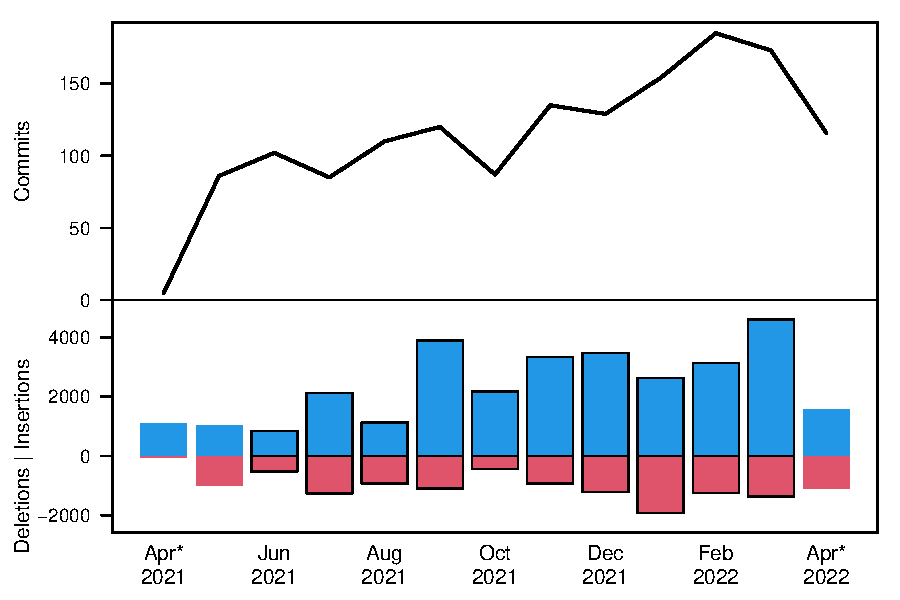
\includegraphics[width=0.57\textwidth]{svnplot_mon42}
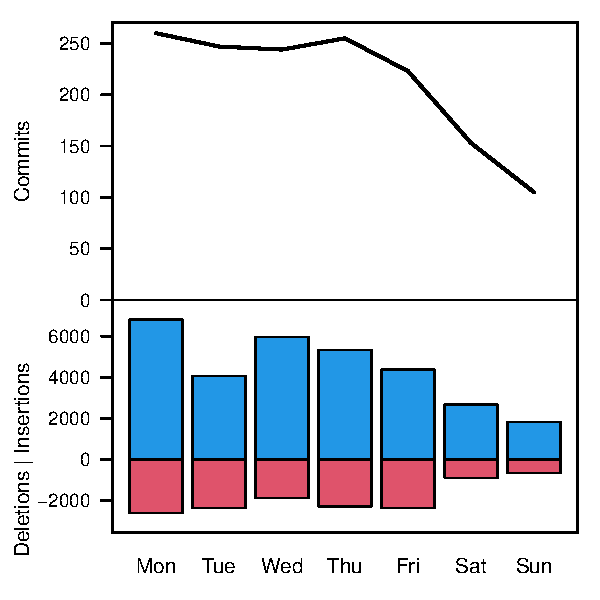
\includegraphics[width=0.38\textwidth]{svnplot_wd42}
\caption{Commit statistics by month (left) and weekday (right) during
R~4.2.0 development.  *Counts for April 2021 represent early work on the
\emph{R-groups} branch.
May 2021 and April 2022 are partial months impacted by the release dates.}
\label{fig:svn42}
\end{figure}


\section{Acknowledgements}
Tomas Kalibera's work on the article and R development has received funding
from the Czech Ministry of Education, Youth and Sports from the Czech
Operational Programme Research, Development, and Education, under grant
agreement No.CZ.02.1.01/0.0/0.0/15\_003/0000421, from the European Research
Council (ERC) under the European Union's Horizon 2020 research and
innovation programme, under grant agreement No.  695412, and from the
National Science Foundation award 1925644.

\begin{samepage}
\address{Tomas Kalibera \\
  Czech Technical University, Czech Republic \\
  \email{Tomas.Kalibera@R-project.org}}

\address{Sebastian Meyer \\
  Friedrich-Alexander-Universit\"at Erlangen-N\"urnberg, Germany \\
  \email{Sebastian.Meyer@R-project.org}}

\address{Kurt Hornik \\
  WU Wirtschaftsuniversit\"at Wien, Austria \\
  \email{Kurt.Hornik@R-project.org}}

\end{samepage}
